% ===================================================================================================
\chapter{Simulations}
% ===================================================================================================

We have studied isotope exchange in four common crystallographic defect systems in tungsten. 
Regardless of the simulated defect, each simulation followed the same general pattern. 
First, a simulation cell of bulk W containing the defect was created and allowed to reach a minimum energy configuration by first using numerical minimization and then relaxation through repeatedly heating and cooling the system during short MD cycles. 
The method of energy minimzation used in all simulations is a Polak-Ribi\`{e}re conjugate gradient algorithm \cite{polak1969note}, used to iteratively adjust atom coordinates until a local energy minimum was found. 

After the initial relaxation, the defect was saturated with T during a 10...200 ns MD run and the excess was removed, prior to adding H to random TIS positions around the bulk material. 
Isotope exchange is then simulated by running MD for a total simulation time of 100...1450 ns. 
Periodic boundaries are applied in all directions and the pressure and temperature are controlled using a Nos\'{e}-Hoover thermostat and barostat, emulating an isothermal-isobaric ensemble. 
In a real world situation, a T atom leaving a defect and diffusing far away will very unlikely return to the same defect, instead of getting caught in another defect or leaving the material through a surface. 
Due to the periodic boundaries, however, this behavior is not seen as the T atom exiting the cell simply returns from the opposite side. 
T counter this, the simulation is performed in intervals of 5 ps (5000 time steps) and between each interval, any T atoms having moved 'far away' are removed from the simulation. 
This decision is made based on the current distance of each T atom from its initial position. 
If the distance exceeds a threshold of $d_{\rm{rmv}} =$ 14 \AA, i.e. ca 4.5 unit cells, the T atom is considered to have left the system. 




% --------------- IsoEx MD ------------------------------------------------------------------------------------
\begin{figure}
\begin{center}
% Define block styles
\tikzset{
decision/.style = {diamond, draw, fill=green!40, 
    text width=4.5em, text badly centered, node distance=3cm, inner sep=0pt},
block/.style = {rectangle, draw, fill=cyan!30, 
    text width=12em, text centered, rounded corners, minimum height=2em},
smallblock/.style = {block, text width=5em},
cloud/.style = {draw, ellipse,fill=red!20, node distance=3cm,
    minimum height=2em}
    }
\begingroup  % compress equations
\medmuskip=2mu
\thinmuskip=1mu
\thickmuskip=2mu
\begin{tikzpicture}
\matrix (m)[matrix of nodes, column  sep=0.0cm,row  sep=5mm, align=center, nodes={rectangle,draw, anchor=south} ]{
   |[block] (initI)| {Create simulation cell containing defect} & \\
   |[block] (initII)| {Relax \& add hydrogen} & \\
    |[block] (MD)| {Run MD for 5000 time steps}          &  \\
    |[block] (Calcd)| {Calculate $d_i$}          &  \\
   |[decision] (IsOut)| {$d_i > d_{\rm{rmv}}$?}              &  \\
       & |[smallblock] (Rmv)| {Remove $i$th T atom}         &  \\
   |[decision] (IsEnd)| {End condition reached?}              &  \\
   |[block] (End)| {Save results \& quit}   & \\
};
\path [>=latex,->] (initI) edge (initII);
\path [>=latex,->] (initII) edge (MD);
\path [>=latex,->] (MD) edge (Calcd);
\path [>=latex,->] (Calcd) edge (IsOut);
\draw [>=latex,->] (IsOut.east) -| node[above, near start] {yes} (Rmv.north);
\draw [>=latex,->] (IsOut.south) -- node[right] {no}(IsEnd);
\draw [>=latex,->] (Rmv.south) |- (IsEnd.north);
\draw [>=latex,->] (IsEnd.west) -- node[above] {no} ++(-2,0cm) |- (MD.west);
\draw [>=latex,->] (IsEnd.south) -- node[right] {yes}(End);
\end{tikzpicture}
\endgroup
\caption{A flowchart representation of the isotope exchange simulations. Variable $d_i$ refers to the distance between current and initial point of T atom $i$.} 
\label{Fig:isoExSimus}
\end{center}
\end{figure}


% ---------------------------------------------------------------------------------------------------
\section{Vacancies}
% ---------------------------------------------------------------------------------------------------
In the vacancy case, a monovacancy was created by removing the middlemost W atom of a $10\times 10 \times 10$ unit cell (2000 atom) W lattice. 
As seen in fig. (\ref{Fig:monovac_system}), six T atoms were then added to the vacancy at their lowest energy positions \cite{heinolaTungstenDFT}, i.e. at the octahedral interstitial sites, forming a square bipyramid. 
A total of 19 H atoms were then deposited to randomly chosen tetragonal interstitial sites around the simulation W lattice, bringing the (H+T)/W ratio to 0.0125. 
The T/H ratio, on the other hand, is 0.32.

A divacancy system was constructed in a similar fashion by removing two neighboring W atoms and adding a total of 10 T atoms to the defect.

\begin{figure}[!ht]
\center
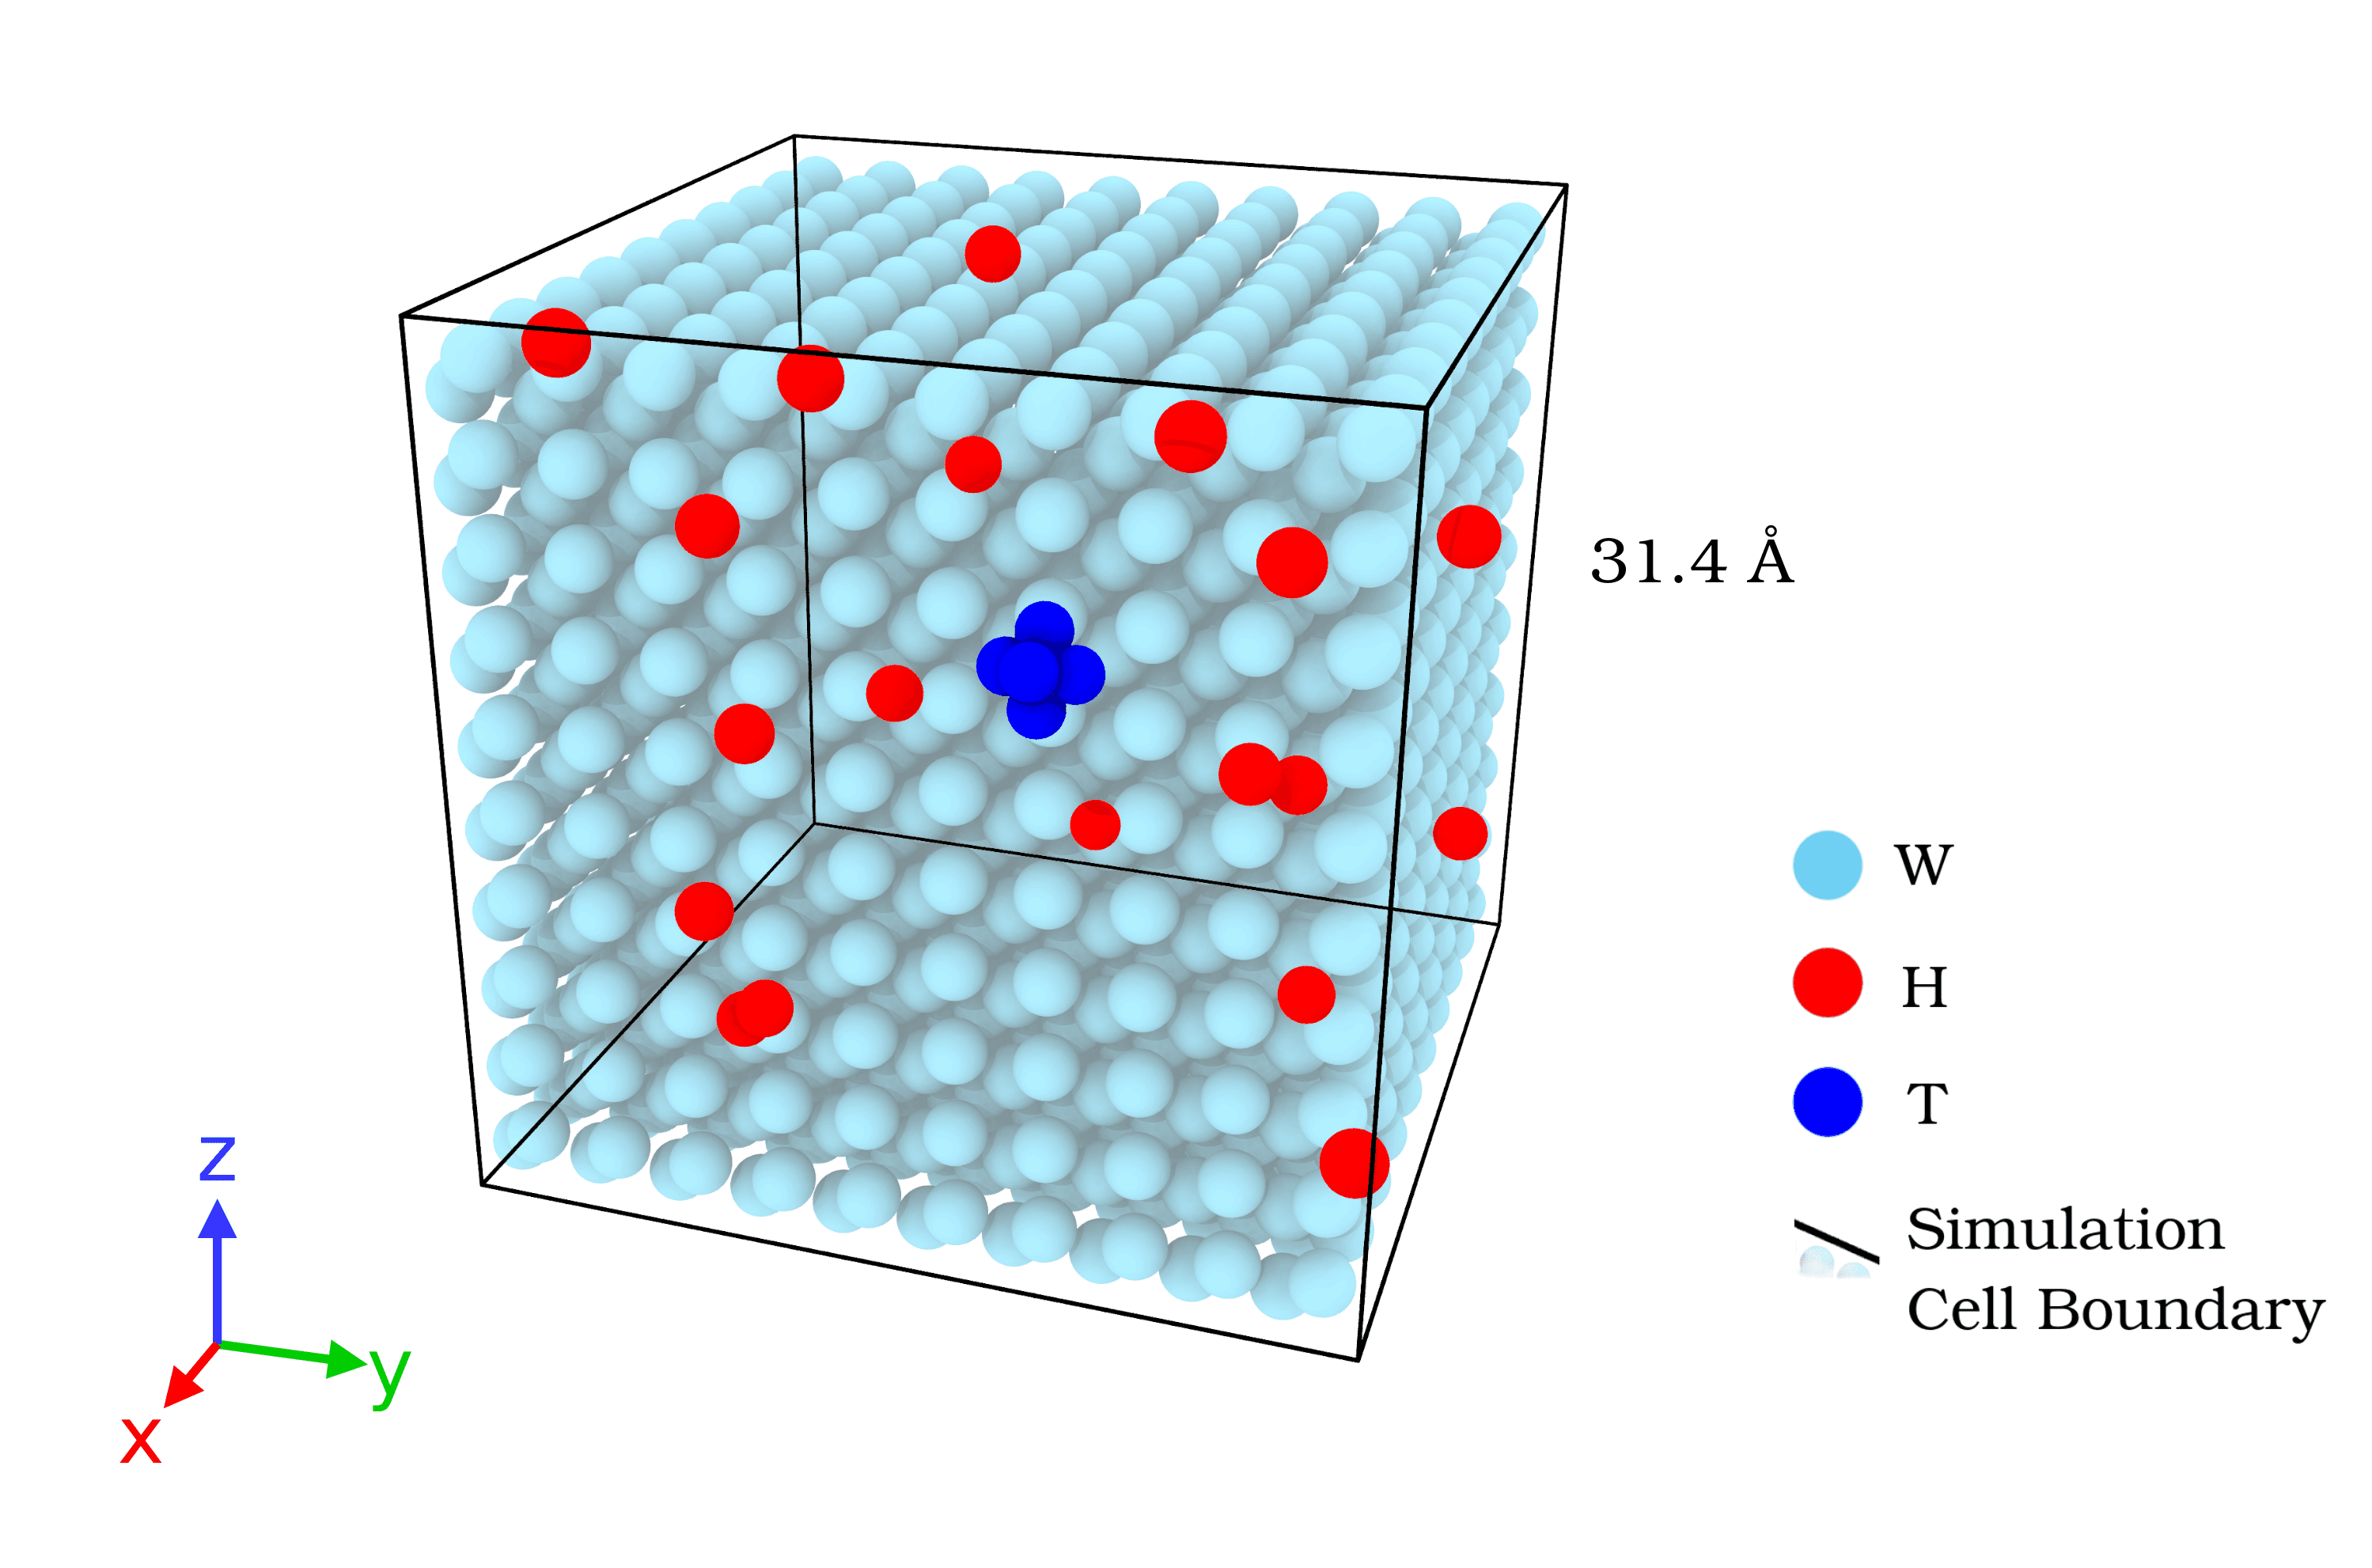
\includegraphics[width=0.7\linewidth]{1Vac_system.png}
\caption{The initial state of the simulation cell used in the monovacancy simulations. 
The W atoms are rendered translucent to display the positions of the hydrogen isotopes.}
\label{Fig:monovac_system}
\end{figure}

% ---------------------------------------------------------------------------------------------------
\section{Dislocations}
% ---------------------------------------------------------------------------------------------------
In the dislocation case, we have created a 1/2\hkl[1 1 1]\hkl{1 0 0} edge dislocation, in a $109.0 \times 136.8 \times 18.4$ $\AA^3$ tungsten super cell with the $x$, $y$ and $z$ axes oriented along the crystal directions  \hkl[1 1 1], \hkl[1 1 -2] and \hkl[-1 1 0] respectively, as shown in fig. (\ref{Fig:disloc_system}). 
The supercell was then divided into three equally thick slices, parallel to the $xz$ plane and a dislocation introduced through the addition of a \hkl{1 1 1} atom plane (parallel to the $yz$ plane) from to the middlemost slice. 
In order to facilitate the formation of a natural dislocation and to enable the use of periodical boundary conditions, the atom positions in the middle slice were finally compressed slightly.

% [Skiss of the dislocation manufacturing process?]

\begin{figure}[!ht]
\center
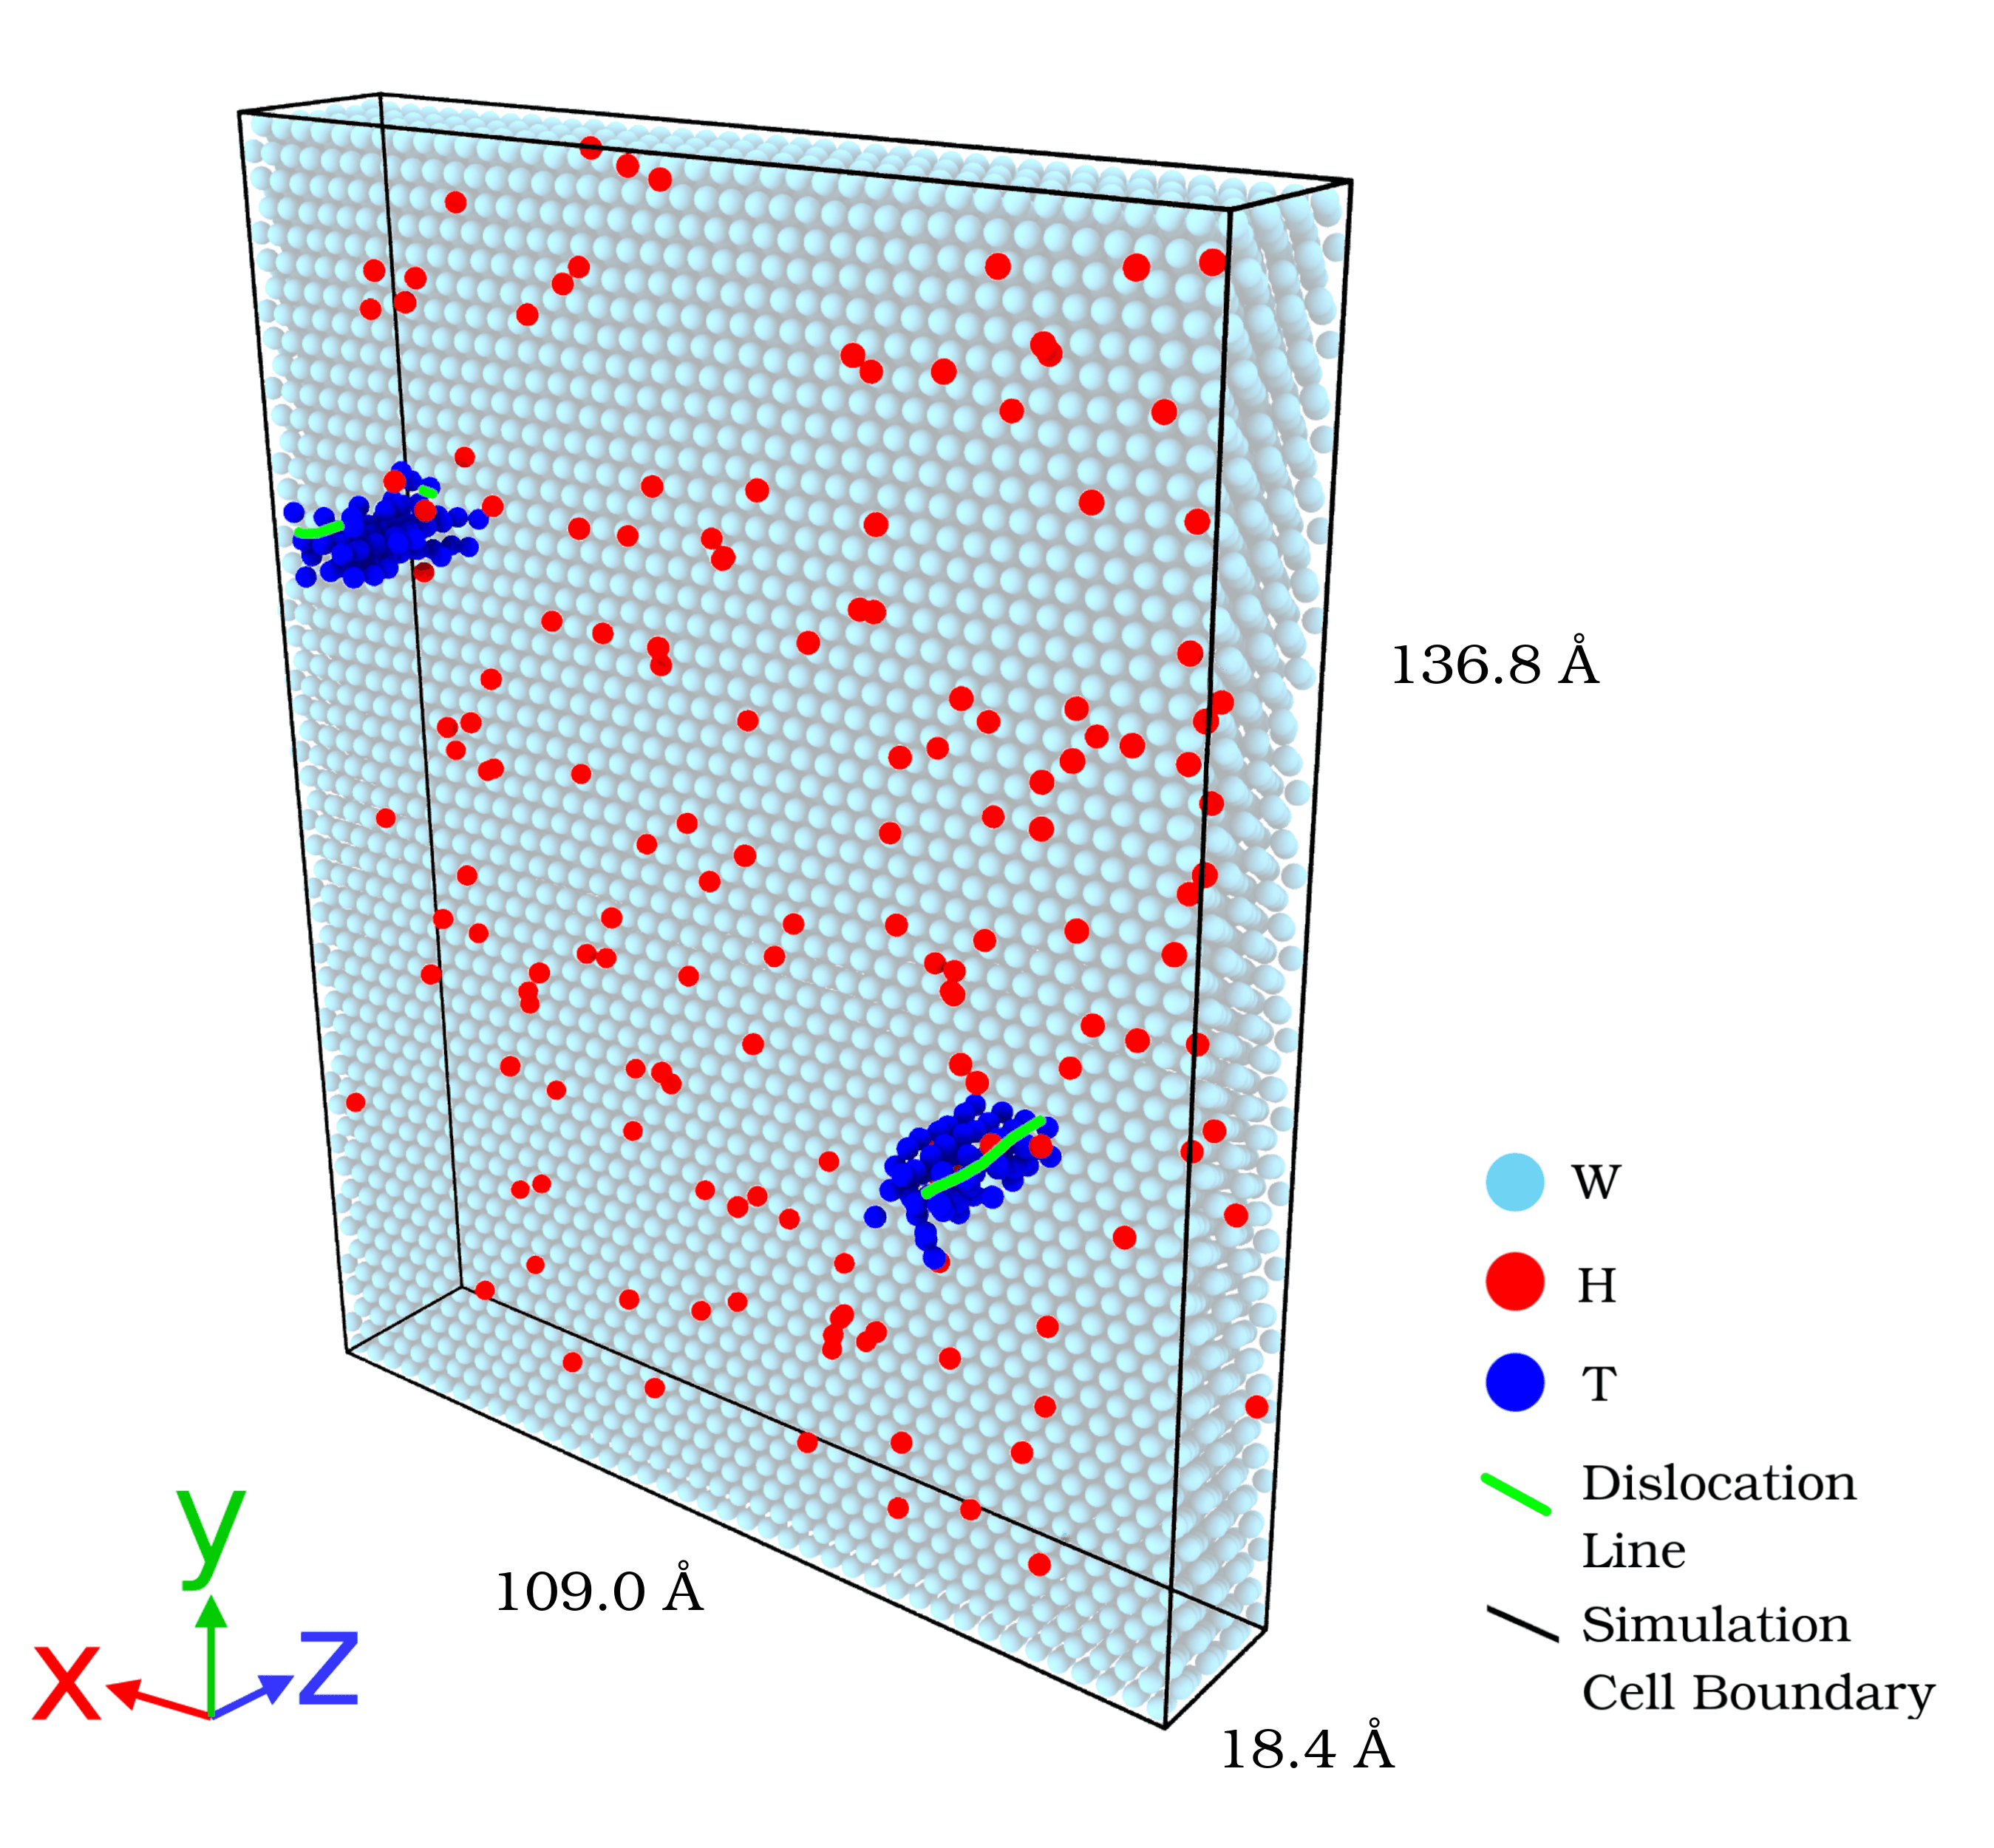
\includegraphics[width=0.7\linewidth]{disloc_system.png}
\caption{The initial state of the simulation cell used in the dislocation simulations. 
The W atoms are rendered translucent to display the positions of the hydrogen isotopes. 
The dislocation, together with its periodic images, is visualized using a defect mesh.}
\label{Fig:disloc_system}
\end{figure}

% ---------------------------------------------------------------------------------------------------
\section{Grain Boundaries}
% ---------------------------------------------------------------------------------------------------
% $\Sigma$5\hkl{310}/\hkl[001]
For simulating isotope exchange in W grain boundaries, we used a system containing an arbitrarily chosen \hkl(310)\hkl[001] tilt grain boundary. The simulation cell was created by growing together two separate tungsten lattices, each rotated through $\pm18.43^\circ$, respectively, around the $z$-axis. 
The $x$-axes of the lattices now point along directions of \hkl<310> and we have a system with a periodicity of $\sqrt{10}~a$ along the $x$- and $y$-axes, and $a$ along the $z$-axis. 
In order to minimize the number of atoms needed to simulate the system we can set $y >> x \approx z$ and again use periodic boundaries.

% Zhou_2009_H_behaviour_in_W_grain_boudnary_FP.pdf

\begin{figure}[!ht]
\center
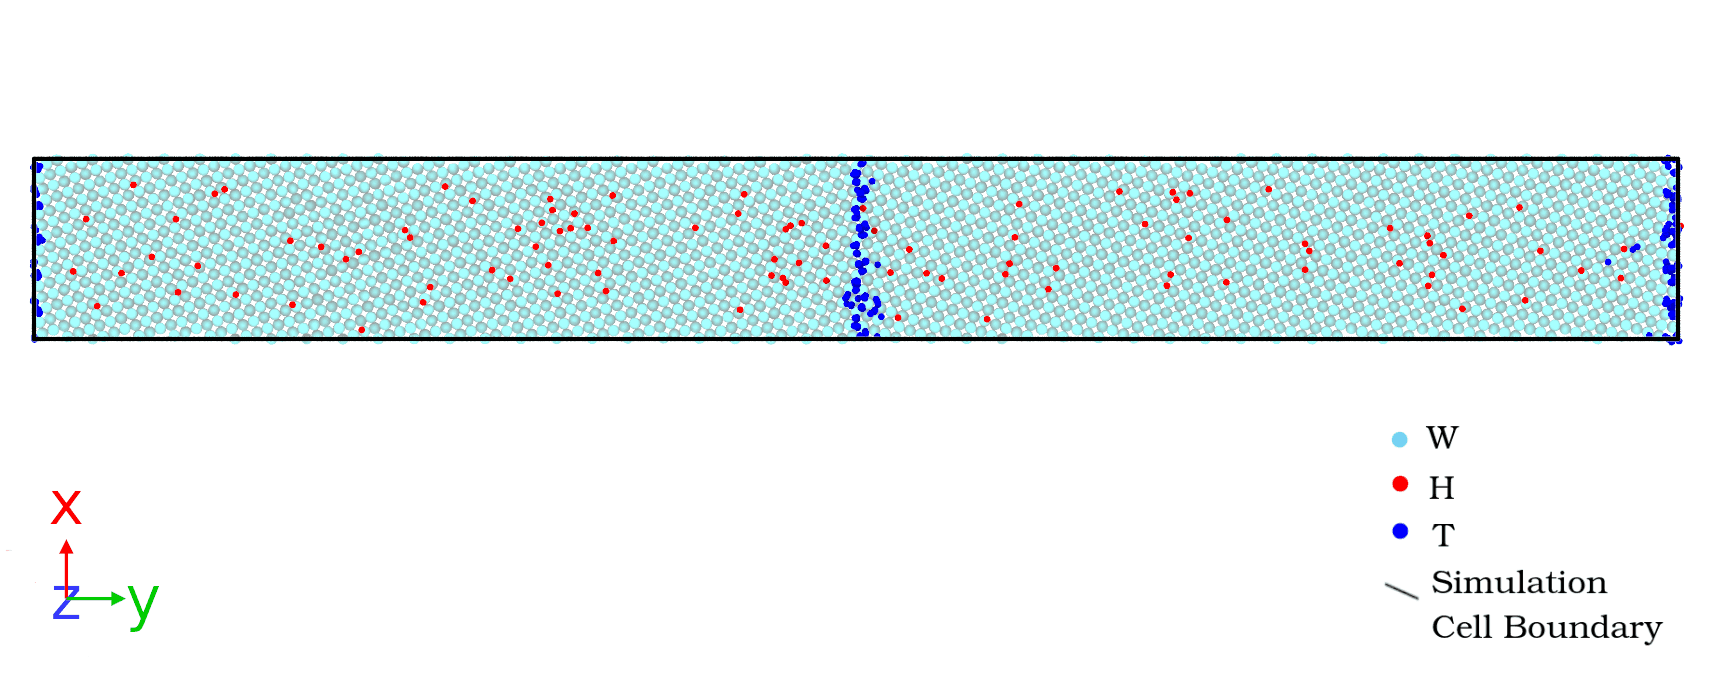
\includegraphics[width=0.94\linewidth]{GB_system.png}
\caption{The initial state of the simulation cell used in the grain boundary simulations. 
The W atoms are rendered translucent to display the positions of the hydrogen isotopes.}
\label{Fig:GB_system}
\end{figure}

% ---------------------------------------------------------------------------------------------------
%\section{Impurities}
% ---------------------------------------------------------------------------------------------------

